\section{Fast Fourier Transform}

\begin{bigidea}
The fast Fourier transform (FFT) is an algorithm for efficiently computing the DFT.
\end{bigidea}

\begin{note}
Sound signals are commonly sampled at 44.1 kHz (see \href{https://en.wikipedia.org/wiki/Sampling_(signal_processing)#Audio_sampling}{Wikipedia: Audio sampling}). Therefore computing the DFT for a one second sound signal requires the Fourier matrix $F_N$ for $N=44100$ which has $44100^2 \approx 2\text{ billion}$ entries. Yikes! We need an efficient algorithm to compute the DFT in practice.
\end{note}

\begin{theorem}
Let $\bs{x} = \begin{bmatrix} x_0 & x_1 & \cdots & x_{N-1} \end{bmatrix}^T$ be a signal of length $N$ (and assume $N$ is even). Then
$$
\mathrm{DFT}(\bs{x}) =
\renewcommand{\arraystretch}{1.25}
\left[ \begin{array}{c}
\mathrm{DFT}(\bs{x}_{\text{even}}) + D_N \mathrm{DFT}(\bs{x}_{\text{odd}}) \\
\mathrm{DFT}(\bs{x}_{\text{even}}) - D_N \mathrm{DFT}(\bs{x}_{\text{odd}})
\end{array} \right]
=
\left[ \begin{array}{rr} I & D_N \\ I & - D_N \end{array} \right]
\left[ \begin{array}{l}
\mathrm{DFT}(\bs{x}_{\text{even}}) \\
\mathrm{DFT}(\bs{x}_{\text{odd}})
\end{array} \right]
\renewcommand{\arraystretch}{1}
$$
where $\bs{x}_{\text{even}}$ and $\bs{x}_{\text{odd}}$ are vectors of length $N/2$ consisting of the even and odd indices respectively
$$
\bs{x}_{\text{even}} = \begin{bmatrix} x_0 \\ x_2 \\ \vdots \\ x_{N-2} \end{bmatrix}
\hspace{10mm}
\bs{x}_{\text{odd}} = \begin{bmatrix} x_1 \\ x_3 \\ \vdots \\ x_{N-1} \end{bmatrix}
$$
and
$$
D_N = \begin{bmatrix} 1 & & & \\ & \omega_N^{-1} & & \\ & & \ddots & \\ & & & \omega_N^{-(N/2-1)} \end{bmatrix}
$$

\begin{proof}
Let $\bs{y} = \mathrm{DFT}(\bs{x})$, look at the $k$th entry of $\bs{y}$ and split the sum into the even and odd terms
\begin{align*}
\bs{y}[k] &= \langle \bs{x} , \bs{f}_k \rangle = \sum_{n=0}^{N-1} x_n \omega_N^{-nk} \\
&= \sum_{m=0}^{N/2-1} x_{2m} \omega_N^{-2mk} + \sum_{m=0}^{N/2-1} x_{2m + 1} \omega_N^{-(2m + 1)k}
\end{align*}
See that $\omega_N^2 = e^{(2 \pi i / N)2} = e^{2 \pi i / (N/2)} = \omega_{N/2}$ and write
$$
\bs{y}[k]= \sum_{m=0}^{N/2-1} x_{2m} \omega_{N/2}^{-mk} + \omega_N^{-k} \sum_{m=0}^{N/2-1} x_{2m + 1} \omega_{N/2}^{-mk}
$$
For $0 \leq k < N/2$, these are the formulas for DFT of vectors of length $N/2$ consisting of the even and odd indices respectively
$$
\bs{x}_{\text{even}} = \begin{bmatrix} x_0 \\ x_2 \\ \vdots \\ x_{N-2} \end{bmatrix}
\hspace{10mm}
\bs{x}_{\text{odd}} = \begin{bmatrix} x_1 \\ x_3 \\ \vdots \\ x_{N-1} \end{bmatrix}
$$
Note that
\begin{align*}
\bs{y}[k + N/2] &= \sum_{m=0}^{N/2-1} x_{2m} \omega_{N/2}^{-m(k + N/2)} + \omega_N^{-(k+N/2)} \sum_{m=0}^{N/2-1} x_{2m + 1} \omega_{N/2}^{-m(k + N/2)} \\
&= \sum_{m=0}^{N/2-1} x_{2m} \omega_{N/2}^{-mk} \underbrace{\omega_{N/2}^{-mN/2}}_{1} + \omega_N^{-k} \underbrace{\omega_N^{-N/2}}_{-1} \sum_{m=0}^{N/2-1} x_{2m + 1} \omega_{N/2}^{-mk} \underbrace{\omega_{N/2}^{-mN/2}}_{1} \\
&= \sum_{m=0}^{N/2-1} x_{2m} \omega_{N/2}^{-mk} - \omega_N^{-k} \sum_{m=0}^{N/2-1} x_{2m + 1} \omega_{N/2}^{-mk}
\end{align*}
which again are the DFTs of the even and odd parts of $\bs{x}$. Put these formulas for $\bs{y}$ together to get
$$
\bs{y} = \mathrm{DFT}(\bs{x}) =
\renewcommand{\arraystretch}{1.25}
\left[ \begin{array}{c}
\mathrm{DFT}(\bs{x}_{\text{even}}) + D_N \mathrm{DFT}(\bs{x}_{\text{odd}}) \\
\mathrm{DFT}(\bs{x}_{\text{even}}) - D_N \mathrm{DFT}(\bs{x}_{\text{odd}})
\end{array} \right]
\renewcommand{\arraystretch}{1}
$$
where
$$
D_N = \begin{bmatrix} 1 & & & \\ & \omega_N^{-1} & & \\ & & \ddots & \\ & & & \omega_N^{-(N/2-1)} \end{bmatrix}
$$
\end{proof}
\end{theorem}

\begin{note}
This form of the fast Fourier transform is called the \href{https://en.wikipedia.org/wiki/Cooley–Tukey_FFT_algorithm}{Cooley-Tukey algorithm}. The point is that the DFT computation for a vector of length $N$ can be compute by the DFT of two smaller vectors of length $N/2$ which is faster! And we can keep applying the formulas for smaller and smaller vectors until we are computing the DFT for vectors of size 2 only (if $N$ is a power of 2). For example, to compute $\mathrm{DFT}(\bs{x})$ for $\bs{x} \in \mathbb{C}^8$ we visualize the procedure

\begin{center}
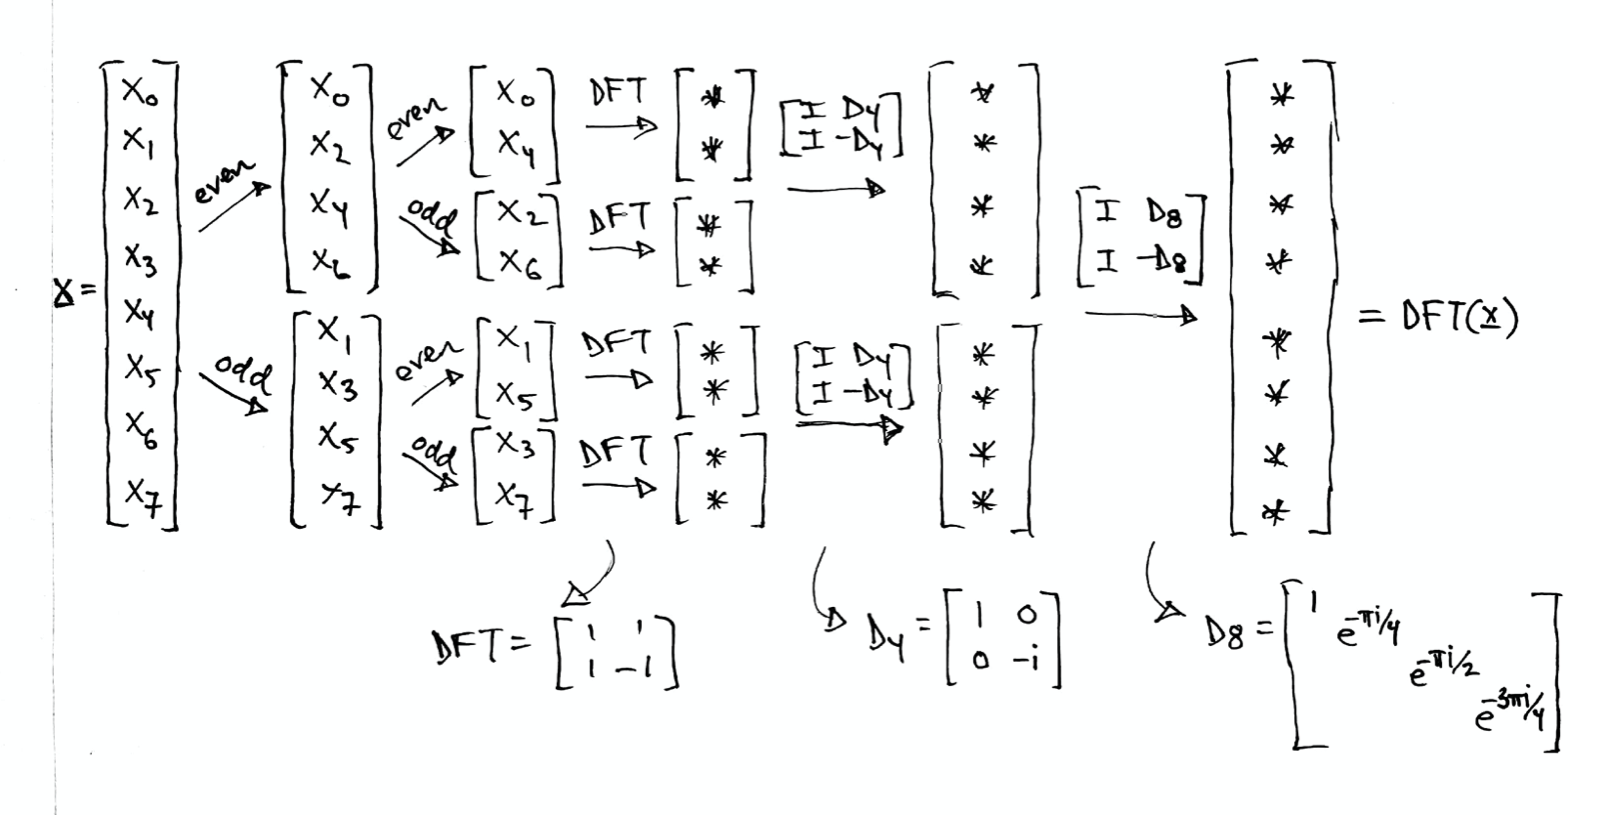
\includegraphics[width=6in]{04_04_fft.png}
\end{center}
\end{note}

\begin{example}
Use the FFT to compute the DFT of the signal
$$
\bs{x} = \begin{bmatrix} 1 & 1 & 1 & 1 & -1 & -1 & -1 & -1 \end{bmatrix}^T
$$
The symmetry in the signal reduces the number of computations even further
$$
\begin{array}{cc}
\begin{array}{c}
\begin{bmatrix} x_0 \\ x_4 \end{bmatrix} = \left[ \begin{array}{r} 1 \\ -1 \end{array} \right] \stackrel{\mathrm{DFT}}{\longrightarrow} \left[ \begin{array}{r} 0 \\ 2 \end{array} \right] 
\vspace{2mm} \\
\begin{bmatrix} x_2 \\ x_6 \end{bmatrix} = \left[ \begin{array}{r} 1 \\ -1 \end{array} \right] \stackrel{\mathrm{DFT}}{\longrightarrow} \left[ \begin{array}{r} 0 \\ 2 \end{array} \right]
\end{array}
&
\longrightarrow
\left[ \begin{array}{c}
\left[ \begin{array}{r} 0 \\ 2 \end{array} \right] + \left[ \begin{array}{rr} 1 & \\ & -i \end{array} \right] \left[ \begin{array}{r} 0 \\ 2 \end{array} \right] \vspace{2mm} \\
\left[ \begin{array}{r} 0 \\ 2 \end{array} \right] - \left[ \begin{array}{rr} 1 & \\ & -i \end{array} \right] \left[ \begin{array}{r} 0 \\ 2 \end{array} \right]
\end{array} \right]
=
\left[ \begin{array}{c} 0 \\ 2-2i \\ 0 \\ 2+2i \end{array} \right]
\vspace{2mm} \\
\begin{array}{c}
\begin{bmatrix} x_1 \\ x_5 \end{bmatrix} = \left[ \begin{array}{r} 1 \\ -1 \end{array} \right] \stackrel{\mathrm{DFT}}{\longrightarrow} \left[ \begin{array}{r} 0 \\ 2 \end{array} \right]
\vspace{2mm} \\
\begin{bmatrix} x_3 \\ x_7 \end{bmatrix} = \left[ \begin{array}{r} 1 \\ -1 \end{array} \right] \stackrel{\mathrm{DFT}}{\longrightarrow} \left[ \begin{array}{r} 0 \\ 2 \end{array} \right]
\end{array}
&
\longrightarrow
\left[ \begin{array}{c}
\left[ \begin{array}{r} 0 \\ 2 \end{array} \right] + \left[ \begin{array}{rr} 1 & \\ & -i \end{array} \right] \left[ \begin{array}{r} 0 \\ 2 \end{array} \right] \vspace{2mm} \\
\left[ \begin{array}{r} 0 \\ 2 \end{array} \right] - \left[ \begin{array}{rr} 1 & \\ & -i \end{array} \right] \left[ \begin{array}{r} 0 \\ 2 \end{array} \right]
\end{array} \right]
=
\left[ \begin{array}{c} 0 \\ 2-2i \\ 0 \\ 2+2i \end{array} \right]
\end{array}
$$
We can write the matrix $D_8$ as
$$
D_8 = \left[ \begin{array}{rrrr} 1 & & & \\ & e^{- \pi i /4} & & \\ & & e^{- \pi i /2} & \\ & & & e^{- 3\pi i /4} \end{array} \right]
= \left[ \begin{array}{rrrr} 1 & & & \\ & \frac{1-i}{\sqrt{2}} & & \\ & & -i & \\ & & & \frac{-1-i}{\sqrt{2}} \end{array} \right]
$$
and then compute
$$
\mathrm{DFT}(\bs{x}) =
\left[
\begin{array}{c}
\left[ \begin{array}{c} 0 \\ 2-2i \\ 0 \\ 2+2i \end{array} \right]
+
\left[ \begin{array}{rrrr} 1 & & & \\ & \frac{1-i}{\sqrt{2}} & & \\ & & -i & \\ & & & \frac{-1-i}{\sqrt{2}} \end{array} \right]
\left[ \begin{array}{c} 0 \\ 2-2i \\ 0 \\ 2+2i \end{array} \right]
\vspace{2mm} \\
\left[ \begin{array}{c} 0 \\ 2-2i \\ 0 \\ 2+2i \end{array} \right]
-
\left[ \begin{array}{rrrr} 1 & & & \\ & \frac{1-i}{\sqrt{2}} & & \\ & & -i & \\ & & & \frac{-1-i}{\sqrt{2}} \end{array} \right]
\left[ \begin{array}{c} 0 \\ 2-2i \\ 0 \\ 2+2i \end{array} \right]
\end{array}
\right]
=
\left[ \begin{array}{c} 0 \\ 2 - 2 \left( \sqrt{2} + 1 \right) i \\ 0 \\ 2 - 2 \left( \sqrt{2} - 1 \right) i \\ 0 \\ 2 + 2 \left( \sqrt{2} - 1 \right) i \\ 0 \\ 2 + 2 \left( \sqrt{2} + 1 \right) i  \end{array} \right]
$$
\end{example}
